\chapter{Fundamentos teóricos}
El presente capítulo abarca los principales temas que se abordan a lo largo de la investigación. Se detalla qué es un sistema de capacitación automatizado, su importancia, sus tipos de preguntas y los modelos de calificación que siguen. Además, se plantea el concepto de sistemas expertos, junto a sus características más notables y su importancia. También estarán explicadas algunas de las funcionalidades del Sistema de Entrenamiento SECPROIT, sus componentes y rendimiento.
Al final del capítulo se observan conclusiones parciales a modo de resumen del mismo.

%%%%%%%%%%%%%%%%%%%%%%%%%%%%%%%%
\section{Sistemas de capacitación laboral}
La capacitación laboral es un método aplicado por las empresas para que su personal adquiera nuevos conocimientos profesionales. Por lo general, se produce ante un ascenso o incorporación, aunque no son los únicos motivos. Busca perfeccionar al colaborador en su puesto laboral, en función de las necesidades de su empresa. Es un proceso estructurado con metas bien definidas. Surge en el mundo como respuesta a la necesidad de mejorar permanentemente la calidad y formación de recursos humanos. Lo ideal es que se desarrolle de forma continua, ya que la constante formación del personal deriva en resultados positivos tanto para el grupo de trabajo como para la organización en la que se realiza \cite{Denby2010}.

\subsection{Características}
Un sistema de capacitación puede ofrecer diferentes aplicaciones en función del modelo de negocio que utilice. Su versatilidad permite adaptarse a las necesidades particulares de cada sector. Sin embargo, según \cite{GarciaPaez2022}, la mayoría de los sistemas contienen las siguientes características:

\begin{itemize}
\item Son capaces de gestionar los distintos cursos impartidos, la asistencia y la inversión en formación de la empresa.
\item Asignan a los empleados que deberán asistir y los profesionales responsables de analizar sus resultados.
\item Detectan las carencias formativas del personal antes de que influyan en el desarrollo del trabajo.
\item Clasifican las distintas actividades formativas en base a su categoría y catálogo.
\item Registran y consultan el progreso del aprendizaje de los empleados en tiempo real.
\end{itemize}

\subsection{Importancia de una buena capacitación}
La capacitación laboral juega un papel primordial para el logro de tareas y proyectos, dado que es el proceso mediante el cual los trabajadores adquieren conocimientos, herramientas, habilidades y actitudes para interactuar de forma correcta y segura en el entorno laboral. Entre los principales beneficios que aporta, según \cite{SistemasCapAsistidos}, se destacan:

\begin{itemize}
\item Calidad y mejora en el resultado de las tareas.
\item Reducción en tiempos y supervisión.
\item Solución de problemas con diferentes visiones.
\item Sensibilización ante nuevos retos.
\item Desarrollo ético y motivación del personal.
\item Seguridad y autoestima en los trabajadores.
\item Mayor especialización.
\end{itemize}

\subsection{Proceso de evaluación}
La evaluación de una capacitación no puede depender de un solo instrumento o técnica, ya que de esa forma solo se mide un tipo de aprendizaje. Los criterios para calificar que se designen, serán los porcentajes de valor que se establezcan a cada resultado de las actividades realizadas, y a su resultado final. Se debe tomar en cuenta tanto la exactitud de la respuesta, como el proceso que se siguió para llegar a la misma, así como la cantidad de intentos necesarios utilizados para hallar la solución \cite{CapTrabajadores}.

Una evaluación posee dos objetivos principales: analizar en qué medida se han cumplido los objetivos y proporcionar la reflexión de los que realizaron el entrenamiento en torno a su propio proceso de aprendizaje (metacognición). Analizar el cumplimiento de los objetivos permite detectar posibles fallas en el proceso y poder superarlas \cite{EtapasEntrenamiento}.

A modo de resumen, para obtener una correcta evaluación se deben tener en cuenta tantas herramientas como parámetros influyan.

\subsection{Fases en un proceso de evaluación de conocimiento}
Un proceso de evaluación de conocimiento, debe estar integrado por cinco etapas (Figura \ref{fig:etapasEval}), asegura \cite{EtapasEntrenamiento}. Cada una de ellas, va a marcar un conjunto de acciones, que al final se interpretarán como un buen entrenamiento:

\begin{enumerate}
\item Recogida de datos: es la recopilación sistemática de toda la información a lo largo del proceso completo de enseñanza-aprendizaje. La información recogida debe tener concordancia con los objetivos trazados, ser suficiente, representativa, relevante y ponderada, en función del peso otorgado a cada uno de los objetivos. En los sistemas en línea estas posibilidades de registrar evidencias son inmensas.
\item Puntuación de las pruebas: se realiza una vez medidos, de manera cuantitativa o cualitativa, los distintos bloques de información, con las ponderaciones, criterios e indicadores que se hayan establecido.
\item Juicio de valor: puede hacerse limitándose a criterios de grupo (evaluación normativa), refiriéndose a criterios de superación de objetivos y contenidos (evaluación de criterio), o teniendo en cuenta la personalidad, posibilidades y limitaciones del propio sujeto del aprendizaje (evaluación personalizada).
\item Toma de decisiones: habitualmente denominada calificación, se basa en la decisión a partir del resultado. Trae consigo una serie de consecuencias personales, administrativas, económicas y laborales. La acción resultante influye directamente en el adiestrado.
\item Información a los interesados: es la etapa final, que ha de llegar a diferentes destinatarios, aunque principalmente y de forma adecuada, a los capacitados. Es la confirmación de que concluye el entrenamiento.
\end{enumerate}

\begin{figure}[h]
\centering
 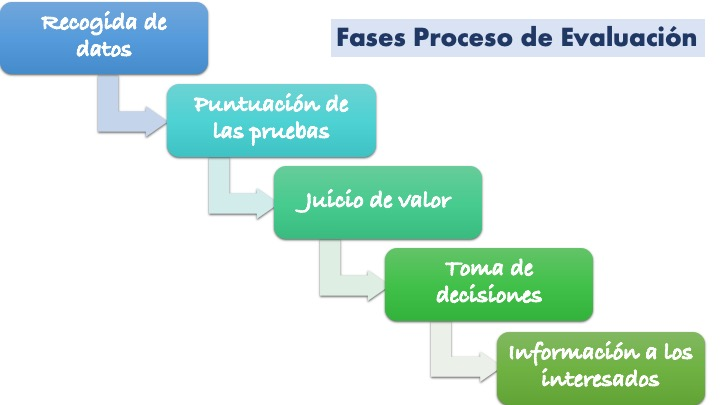
\includegraphics[width=0.5\linewidth]{imagen/FasesEva.jpg}
 \caption{Fases de un proceso de evaluación de conocimiento.}
 \label{fig:etapasEval} 
\end{figure}

\subsection{Proceso de validación de las respuestas}
Una vez terminada la capacitación se deben comprobar cuáles de los resultados obtenidos son correctos y cuáles no. Para ello se deben comparar las respuestas del evaluado con una fuente de confianza, que contenga la información verídica de lo que se está tratando. Estas fuentes de confianza se conocen por el nombre de: bases de conocimiento \cite{SEdiagramas}.

A partir de estas bases se verifica si los datos en las respuestas del evaluado coinciden con la información real contenida. Este proceso puede realizarse tanto de manera manual, semiautomática o automática.

%%%%%%%%%%%%%%%%%%%%%%%%%%%%%%%
\section{Sistemas de capacitación automatizados}
Basándose en el concepto de capacitación, un sistema de capacitación automatizado es un método de enseñanza alternativo creado para el adiestramiento de los trabajadores. Es un software que, principalmente, permite el aprendizaje de los usuarios sin necesidad de una supervisión constante. Por lo general, resulta más efectivo que las prácticas de enseñanza presencial, debido a que el estudiante trabaja solo y puede determinar su propia velocidad de aprendizaje, usando una amplia variedad de herramientas y métodos para la transferencia del conocimiento \cite{CapacitacionAuto}.

A modo de resumen, es un software que brinda una solución de recursos humanos, ayuda en la formación de los trabajadores y aumenta la productividad empresarial.

\subsection{Ventajas}
Un sistema de entrenamiento asistido por computadora (sistema de capacitación automatizado), permite ofrecer el mismo nivel de adiestramiento para cada usuario del sistema, en cuanto a rigor y evaluación. Uno de los problemas principales de la capacitación de los empleados de manera presencial es que las sesiones son frecuentemente inconsistentes y las diferencias en el nivel de habilidad del formador pueden tener un impacto significativo en el éxito del empleado. Al contar con un sistema automatizado, solo se necesita una base de conocimiento para garantizar el mismo nivel de entrenamiento para todos los capacitados \cite{SistemaCapAut}.

\subsection{Desventajas}

\subsection{Tipos de preguntas más utilizadas}
A medida que avanza el tiempo, se generan nuevos métodos de estudio, y con estos, nuevas formas de preguntar y calificar. Sin embargo, a la hora de diseñar un sistema automatizado, no es menos cierto que existen algunas variantes más sencillas y, por ende, más utilizadas. Según \cite{Catadores}, los tipos de preguntas que mayormente se emplean en un sistema de este tipo son:

\begin{itemize}
\item Verdadero o falso: contienen una declaración que se debe indicar si es verdadera o no. Permiten responder en poco tiempo, son fáciles, rápidos de calificar y se corrigen de forma automática.
\item Opción múltiple: se componen de una pregunta (raíz) con múltiples respuestas posibles. Pueden incluir múltiples opciones válidas, en cuyo caso, podrían darse por superada al marcar cualquiera de ellas o cuando se marquen todas. Se caracterizan por ser fáciles y rápidas de calificar, por corregirse automáticamente y utilizarse para evaluar los conocimientos en una amplia gama de contenidos.
\item Emparejar, relacionar u ordenar: por lo general se emparejan cada una de las opciones del primer bloque con las opciones dadas en el segundo bloque, o se ordenan bloques de modo que quede una secuencia correcta de acuerdo a un patrón previamente establecido. Se suelen usar en aquellos cursos donde la adquisición de conocimientos muy detallados es un objetivo importante. Son preguntas fáciles de diseñar, rápidas de calificar y se corrigen automáticamente. Estadísticamente, se tarda más en responder que las preguntas anteriores.
\item Respuesta corta: basta con que se escriban un par de palabras o una frase sencilla. Una alternativa más común a este tipo de preguntas es la de cubrir espacios en blanco con una palabra. Son de gran utilidad a la hora de demostrar los conocimientos basados en hechos o palabras claves. La dificultad para calificarlas depende del estilo que se decida emplear.
\end{itemize}

\subsection{Proceso de validación de las respuestas}
Al tratarse de un sistema de capacitación automatizado, por lo general, el método utilizado para validar las respuestas es el automático. De esta forma se facilita el trabajo para aquellos que deben evaluar a un personal abundante. Según \cite{ExpertSystem}, la manera más efectiva y eficiente de evaluar las respuestas en estos sistemas es mediante el uso de sistemas expertos.

\subsection{Evolución a través de la historia}

%%%%%%%%%%%%%%%%%%%%%%%%%%%%%%%%%
\section{Sistemas expertos}
Los sistemas expertos resuelven problemas que normalmente son solucionados por expertos humanos. Para hacerlo, necesitan acceder a una importante base de conocimiento sobre el dominio, que debe construirse de la manera más eficiente posible. Utilizan uno o más mecanismos de razonamiento, para aplicar este conocimiento a los problemas que se le proponen. Cuentan con un mecanismo para explicar a los usuarios que han confiado en ellos, lo que han hecho y cómo \cite{VonRueden2019}.

Una forma de contemplar los sistemas expertos es que representan la mayor parte de la Inteligencia Artificial (IA) aplicada. Un sistema experto en IA se define como un programa informático que tiene la capacidad de representar y razonar sobre el conocimiento \cite{SEdiagramas}.

\subsection{Componentes}
En \cite{OdhiamboOmuya2021} se comentan los diferentes componentes que integran un sistema experto. Aunque pueden contar con un número mayor, los mínimos requeridos son (Figura \ref{fig:componentesSE}):

\begin{itemize}
\item Motor de inferencia: es el corazón del sistema experto. Su cometido principal es sacar conclusiones aplicando el conocimiento a los datos. Estas conclusiones pueden estar basadas en conocimiento determinista o conocimiento probabilístico.
\item Base de conocimiento: consiste en un conjunto de objetos y un conjunto de reglas que gobiernan las relaciones entre esos objetos. La información que almacena es de naturaleza permanente y estática, es decir, no cambia de una aplicación a otra. Se debe diferenciar entre los datos y el conocimiento. El conocimiento se refiere a afirmaciones de validez general tales como reglas, distribuciones de probabilidad, entre otras. Los datos se refieren a información relacionada con una aplicación en particular.
\item Mecanismo de aprendizaje: controla el flujo del nuevo conocimiento que va del experto humano a la base de conocimiento. El sistema determina qué nuevo conocimiento se necesita, o si el conocimiento es realidad, es decir, si debe incluirse, y en caso necesario incorporar dicho conocimiento.
\item Interfaz de usuario: es la interfaz entre el sistema experto y el usuario. Para que sea efectiva debe incorporar mecanismos para mostrar y obtener información de forma sencilla y agradable.
\end{itemize}

\begin{figure}[h]
\centering
 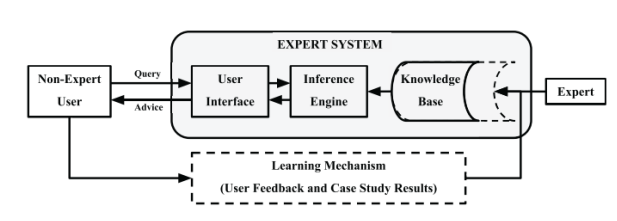
\includegraphics[width=0.8\linewidth]{imagen/ComponentesSE.png}
 \caption{Componentes de un sistema experto.}
 \label{fig:componentesSE} 
\end{figure}

\subsection{Ventajas}
A pesar de sus desventajas, el uso de un sistema experto en cualquier ámbito social resulta favorable de diversas maneras. Según \cite{Mitchell1990}, entre sus ventajas más destacadas se pueden encontrar:

\begin{itemize}
\item No sufre de limitaciones y percances humanos, lo que lo convierte en una herramienta estable y fiable para su entorno.
\item Sus actividades son completamente replicables y siempre contesta de la misma manera a menos que se le cambie el diseño.
\item La velocidad de procesamiento es mayor al de un ser humano.
\item Pueden almacenar su conocimiento para cuando sea necesario aplicarlo.
\item Pueden ser utilizados por personas no especializadas para resolver problemas.
\item Pueden ser usados como sistema de aprendizaje.
\item Al evaluar el costo total del empleo de esta tecnología, la replicabilidad y estabilidad, asociado a la seguridad que provee, resulta una ecuación favorable, aún considerando que las inversiones iniciales pueden ser
relativamente elevadas.
\end{itemize}

\subsection{Desventajas}
A pesar de las ventajas que puede proporcionar el uso de sistemas expertos, su tecnología novedosa trae consigo ciertas desventajas. En \cite{SystemExpertsEstudents} se mencionan algunas de ellas:

\begin{itemize}
\item Para actualizarlos se necesita de reprogramación, siendo una de sus limitaciones más acentuadas.
\item Son poco flexibles a cambios y de difícil acceso a información no estructurada.
\item Poseen elevado costo en dinero y tiempo. 
\item Carecen de sentido común (no hay nada obvio).
\item No se puede mantener una conversación informal con ellos.
\item Es muy complicado que aprendan de sus errores o de errores ajenos.
\item No son capaces de distinguir cuáles son las cuestiones relevantes de un
problema y separarlas de cuestiones secundarias.
\end{itemize}

Sin embargo, estos problemas no solo los presentan los sistemas expertos. La Inteligencia Artificial (IA) aún no ha podido desarrollar sistemas que
sean capaces de resolver problemas de manera general o de aplicar el sentido común para resolver situaciones complejas. Es por ello que, a pesar de sus desventajas, los sistemas expertos son considerados una gran ayuda y un enorme avance, en especial, en el campo de los sistemas de capacitación \cite{Barham2019}.

%%%%%%%%%%%%%%%%%%%%%%%%%%%%%%%%%
\section{Sistema de entrenamiento SECPROIT}
En el año 2019 se creó el Sistema Experto para el Control de Procesos Químicos (SECPROIT), que es un sistema diseñado para capacitar a los operarios de la Industria Alimentaria Cubana sobre los diferentes procesos productivos que en ella se realizan. Este sistema fue desarrollado en la Universidad Tecnológica de La Habana José Antonio Echeverría (CUJAE), entre las facultades de Ingeniería Química e Ingeniería Informática. Su objetivo principal es lograr capacitar a los operarios de la industria y, para ello, realiza un conjunto de entrenamientos evaluados por un sistema experto \cite{BasesConocimientoArt}.

\subsection{Funcionamiento}
El sistema SECPROIT está diseñado para capacitar a los trabajadores de las fábricas, a partir de entrenamientos relacionados con los procesos productivos que en ellas se realizan, mediante el uso de sistemas expertos. En este, existen tres roles fundamentales: 

\begin{itemize}
\item Administrador: se encarga del control de los datos del sistema.
\item Especialista: es el responsable de insertar las bases de conocimiento en el sistema y supervisa los resultados obtenidos por los trabajadores de su área laboral.
\item Operario: realiza los entrenamientos.
\end{itemize}

Cada usuario tiene un nombre, una contraseña y un rol, y con cada rol aparecen funcionalidades únicas y específicas. En el caso de los especialistas, para insertar una base de conocimiento deben asociarla a un proceso, y de cada proceso deben registrar el nombre, una imagen si la posee, un fichero tipo \textsl{anm} y un archivo \textsl{drl} \cite{SECPROIT}.

Los ficheros \textsl{anm} contienen los nombres de todas las variables que influyen en el proceso, sus características, las causas que pueden hacer que entren en estado de alarma y las recomendaciones para cada una de las causas descritas. Por otra parte, el archivo \textsl{drl} contiene las reglas que enlazan las variables con sus causas y las causas con sus recomendaciones. Dichas reglas siguen una estructura específica: comienzan con un patrón para el nombre de las reglas, luego presentan los posibles atributos que poseen, las sentencias que se deben cumplir y las acciones que realizar si se cumplen las sentencias (Figura \ref{fig:drools}). Este archivo es lo que se conoce como Motor de Reglas (Drools) \cite{BaseConocimiento}.

\begin{figure}[h]
\centering
 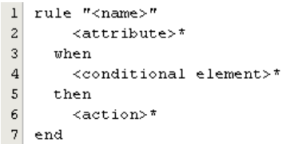
\includegraphics[width=0.5\linewidth]{imagen/EstructuraDRL.png}
 \caption{Estructura de un archivo \textsl{drl}.}
 \label{fig:drools} 
\end{figure}

El operario entrará a realizar aquellos entrenamientos que el especialista haya validado. Una vez comenzada la prueba, deberá señalar de un grupo de variables las que por su estado estén en peligro de inestabilidad. Si ha seleccionado correctamente pasa a la siguiente etapa, donde debe escoger qué causa el estado de las variables que prefirió. Por último deberá seleccionar qué recomendaciones seguir para cada causa que señaló \cite{SECPROIT}.

Este sistema posee un grupo de reportes que facilita la toma de decisiones a partir de los resultados alcanzados. El especialista puede contar con una lista de resultados de cada operario de su área y, de esta forma, se garantiza la selección de los mejores trabajadores a partir de la organización brindada por la lista. También se puede encontrar un listado de los cambios realizados en el sistema, junto con la fecha y el nombre del usuario que lo realizó.

\subsection{Limitaciones actuales del sistema}
Actualmente el sistema SECPROIT posee ciertas limitaciones que impiden que sea implementado en las industrias:

\begin{itemize}
\item La información necesaria para generar los entrenamientos es extraída en todo momento, de forma directa, de los ficheros \textsl{anm} y \textsl{drl}, lo que genera una demora extra en el sistema.
\item Solo existe un método de pregunta.
\item El resultado de un entrenamiento está dado por la cantidad de preguntas correctas que se completaron, sin tener en cuenta el tiempo demorado.
\item La etapa final no se evalúa correctamente ni muestra la puntuación obtenida.
\item Las etapas del entrenamiento se realizan de manera continua, sin posibilidad de pausa.
\item Las etapas aparecen de forma consecutiva, sin importar si la anterior fue aprobada o no (aparecen etapas innecesariamente).
\item Por cada proceso existe un único entrenamiento, lo que limita la capacidad de aprendizaje del trabajador.
\item Las pantallas del sistema son poco intuitivas, con colores oscuros y de diversos tamaños, lo que resulta poco amigable para el usuario que las emplea.
\end{itemize}

%%%%%%%%%%%%%%%%%%%%%%%%%%%%%%%%%
\section{Generador de Bases de Conocimiento}
Como todo sistema experto, el sistema SECPROIT posee un conjunto de bases de conocimiento que, en este caso, fue creada por un Generador de Bases de Conocimiento. Dicho generador fue desarrollado en el año 2018 por la Universidad Tecnológica de La Habana José Antonio Echeverría (CUJAE), entre las facultades de Ingeniería Química e Ingeniería Informática. Es un sistema para facilitar la creación de dichas bases. En él se introducen de manera manual todos los datos relacionados a las variables, causas y recomendaciones de los procesos productivos. Luego deberán inluirse las reglas entre las variables y las causas, y las relaciones entre las causas y las recomendaciones. Una vez completada esta información, de forma semi-automática, se generan los ficheros \textsl{anm} y \textsl{drl} que serán utilizados por el SECPROIT \cite{BaseConocimiento}.

%%%%%%%%%%%%%%%%%%%%%%%%%%%%%%%%%

\section{Conclusiones Parciales}
A partir de la investigación realizada y los aspectos profundizados a lo largo del capítulo:

\begin{itemize}
\item Se hizo un estudio detallado de los sistemas de capacitación existentes, llegando a concluir que, por las condiciones que presentan, el sistema de capacitación que más se ajusta a la Industria Alimentaria Cubana es el digital.
\item Se tuvieron en cuenta todos los detalles de la problemática planteada y, gracias a las similitudes existentes, se concluyó que un sistema experto resulta la herramienta idónea para esta solución.
\item Se analizó con profundidad el sistema SECPROIT para ser tomado como base a la hora de diseñar y programar el nuevo sistema. Será el modelo a seguir y se rectificarán todos las limitaciones existentes en él para esta nueva versión.
\end{itemize}
